\documentclass[crop]{standalone}
\usepackage{tikz}
%\usepackage[]{tikz-3dplot}
\usepackage{pgfplots}
\pgfplotsset{compat=1.15}
\usepackage[]{amsmath}
\usepackage[]{libertine}
\usepackage[libertine]{newtxmath}
\usepackage[]{bm}
\usepackage[]{physics}
% Macros for greek letters in roman style, in math mode
\DeclareRobustCommand{\mathup}[1]{%
\begingroup\ensuremath\changegreek\mathrm{#1}\endgroup}
\DeclareRobustCommand{\mathbfup}[1]{%
\begingroup\ensuremath\changegreek\bm{\mathrm{#1}}\endgroup}


\makeatletter
\def\changegreek{\@for\next:={%
        alpha,beta,gamma,delta,epsilon,zeta,eta,theta,iota,kappa,lambda,mu,nu,%
        xi,pi,rho,sigma,tau,upsilon,phi,chi,psi,omega,varepsilon,varpi,%
    varrho,varsigma,varphi}%
\do{\expandafter\let\csname\next\expandafter\endcsname\csname\next up\endcsname}}
\makeatother

% Define vectors in bold, roman, lowercase font
\newcommand{\vct}[1]{\ensuremath{\mathbfup{\MakeLowercase{#1}}}}

% Define unit vectors in bold, roman, lowercase font, with hats
\newcommand{\uvct}[1]{\ensuremath{\mathbfup{\hat{\MakeLowercase{#1}}}}}

% Define matrices in bold, roman, uppercase font
\newcommand{\mtrx}[1]{\ensuremath{\mathbfup{\MakeUppercase{#1}}}}
\usetikzlibrary{%
    shapes,%
    arrows,%
    patterns,%
    positioning,%
    calc%
}




%\tdplotsetmaincoords{60}{90}

\begin{document}

\tikzstyle{block} = [draw, rectangle, stroke = black!80,fill = gray!15, minimum height = 3em, minimum width = 6em]
\tikzstyle{cloud} = [draw, stroke=black!80, fill=gray!15,ellipse, minimum height = 3em, minimum width = 6em]
\tikzstyle{arr} = [single arrow, draw, ->]

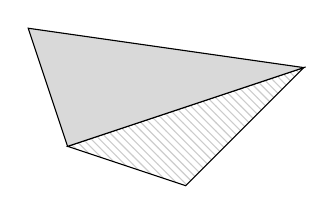
\begin{tikzpicture}%[tdplot_main_coords]
    % Define common vertices
    \coordinate (v1) at (0,1);
    \coordinate (v2) at (3,2);
    % Define differing vertices
    \coordinate (a) at (1.5,0.5);
    \coordinate (b) at (-0.5,2.5);

    % Draw the triangles
    \draw[pattern = north west lines, pattern color = gray!40, stroke = black!80, draw opacity = 1] (v1) -- (v2) -- (a) -- cycle;
    \draw[fill = gray!30, stroke = black!80, draw opacity = 1] (v1) -- (v2) -- (b) -- cycle;
\end{tikzpicture}
\end{document}
